\documentclass[utf8]{beamer}
\usepackage{listings}
\usepackage[russian]{babel}
\usetheme{Malmoe}
\title{Стандартизация в области телекоммуникаций.\newline Передача данных на физическом уровне (I)}
\author {Компьютерные сети и протоколы}
\date{Лекция 2}
\begin{document}
%--------------------------------------------------------------------------------
\begin{frame}
\titlepage
\end{frame}
%--------------------------------------------------------------------------------
\section{Материал прошлой лекции}
%--------------------------------------------------------------------------------
\begin{frame}
\frametitle{Архитектура компьютерных сетей}
\begin{itemize}
 \item Уровневая архитектура
 \begin{itemize}
    \item Разделение функций
    \item Скрытие деталей реализации протоколов
 \end{itemize}
 \item Службы (на основании установления соединения, без установления соединения) -- набор функций, предоставляемых пользователю или вышележащему уровню
 \item Протокол -- набор правил, описывающих формат и назначение кадров, пакетов, или сообщений, которыми обмениваются объекты одного ранга в пределах одного уровня.
\end{itemize}
\end{frame}
%--------------------------------------------------------------------------------
\section{Стандартизация в области телекоммуникаций}
%--------------------------------------------------------------------------------
\subsection{Необходимость стандартизации}
%--------------------------------------------------------------------------------
\begin{frame}
\frametitle{Что такое стандарты?}
\begin{block}{Для чего разрабатываются стандарты?}
Стандарт определяет то, что \emph{необходимо для взаимодействия}.
\begin{itemize}
 \item Например, выбор канальной скорости в IEEE 802.11 стандартом не предусмотрен.
 \item Для рассмотрения вопросов взаимодействия зачастую создаются рабочие группы (WiFi Alliance).
\end{itemize}
\end{block}
\begin{block}{Две категории стандартов}
\begin{itemize}
 \item[de facto] -- стандарты, ставшие такими без предварительного планирования, а благодаря успешной реализации (HTTP, созданный в Церне, Bluetooth, разработанный Ericsson).
 \item[de jure] -- приняты по некоторым законам стандартизации.
\end{itemize}
\end{block}
\end{frame}
%--------------------------------------------------------------------------------
\begin{frame}
\frametitle{Кто пишет стандарты?}
\begin{itemize}
 \item Международные организации по стандартизации, организованные на основании межправительственных договорённостей или добровольно: IEEE, ITU, ISO, IETF.
 \item Деловые организации, образуемые вокруг некоторой технологии (3GPP -- объединение организаций, занимающихся стандартизацией мобильной связи 3G UMTS)
\end{itemize}
\begin{block}{3GPP}
\begin{itemize}
 \item Объединяет 6 организаций по стандартизации (ARIB, ATIS, CCSA, ETSI, TTA, TTC)
 \item Объединяет 4 группы по разработке стандартов (Radio Access Network -- RAN, Service \& System Aspects, Core Network \& Terminals, GSM EDGE RAN)
\end{itemize}
\url{www.3gpp.org}
\end{block}
\end{frame}
%--------------------------------------------------------------------------------
\begin{frame}
\frametitle{Кто нуждается в стандартах?}
\begin{block}{Правительственные и частные организации}
 \begin{itemize}
  \item Права на средства связи принадлежат частным компаниям (США)
  \item Права на средства связи принадлежат Правительству (почти все остальные)
 \end{itemize}
\end{block}
\begin{itemize}
 \item[o] Тенденция к переходу прав частным компаниям.
\end{itemize}
\Large
Необходимость стандартизации на международном уровне.
\end{frame}
%--------------------------------------------------------------------------------
\subsection{Международные организации по стандартизации}
%--------------------------------------------------------------------------------
\begin{frame}
\frametitle{ITU -- Международный Союз Электросвязи}
ITU (МСЭ) основан в 1865 году (стандартизована азбука Морзе). На сегодняшний день состоит из трёх секторов:
 \begin{itemize}
  \item [ITU-T] Телекоммуникационный сектор стандартизации в области систем передачи данных и телефонии.
  \item [ITU-R] Сектор радиосвязи (использование радиочастот).
  \item [ITU-D] Сектор развития. Развитие телекоммуникационных технологий в странах Третьего мира.
\end{itemize}
\begin{block}{Иерархия подразделений}
Сектор $\Rightarrow$ Исследовательская группа $\Rightarrow$ Рабочая группа $\Rightarrow$ Экспертная команда.
\end{block}
\end{frame}
%--------------------------------------------------------------------------------
\begin{frame}
\frametitle{ISO -- Международная организация по стандартизации}
Комитеты $\Rightarrow$ Подкомитеты $\Rightarrow$ Рабочие группы
\begin{itemize}
 \item Более двухсот комитетов
 \item Рабочие группы состоят из ``добровольцев'' -- представителей компаний, чьи продукты должны быть стандартизованы.
 \item Многоэтапная разработка стандартов (Commitee Draft $\rightarrow$ Draft International Standard $\rightarrow$ International Standard)
\end{itemize}
\end{frame}
%--------------------------------------------------------------------------------
\begin{frame}
\frametitle {IEEE -- Институт инженеров по электротехнике и электронике}
\begin{description}
 \item [Комитет 802] в области телекоммуникаций. Образован в феврале 1980 года.
\end{description}
\begin{block}{Рабочие группы комитета 802:}
\begin{itemize}
 \item [802.3] Ethernet -- наиболее распространённая технология проводных ЛВС.
 \item [802.11] WiFi (Wireless Fidelity) -- технология беспроводных ЛВС.
 \item [802.15] Персональные беспроводные сети (Bluetooth).
 \item [802.16] WiMAX -- Городские широкополосные сети.
\end{itemize}
\end{block}
\end{frame}
%--------------------------------------------------------------------------------
\subsection{Стандартизация Интернета}
%--------------------------------------------------------------------------------
\begin{frame}
\frametitle {Стандарты Интернета -- <<Грубый консенсус и работающая программа>>}
\begin{itemize}
 \item [IAB] Internet Activities Board, Совет по деятельности Интернета, создан министерством обороны США после запуска ARPANET. Упорядочение деятельности исследователей и разработчиков ARPANET.
 \item [RFC] Набор технических отчётов (Request For Comments), выпущенных IAB.
 \item [IRTF] Internet Research Task Force, группа исследования Интернета -- результат реорганизации IAB (как и IETF). Задачи долгосрочного развития.
 \item [IETF] Internet Ingineering Task Force, группа проектирования Интернета, решающая краткосрочные инженерные задачи.
 \item [W3C] Консорциум World Wide Web. Решение таких вопросов, как веб-безопасность.
\end{itemize}
\end{frame}
%--------------------------------------------------------------------------------
\section{Теоретические основы передачи данных}
%--------------------------------------------------------------------------------
\begin{frame}	
\frametitle{Представление сигнала в канале передачи данных}
\begin{center}
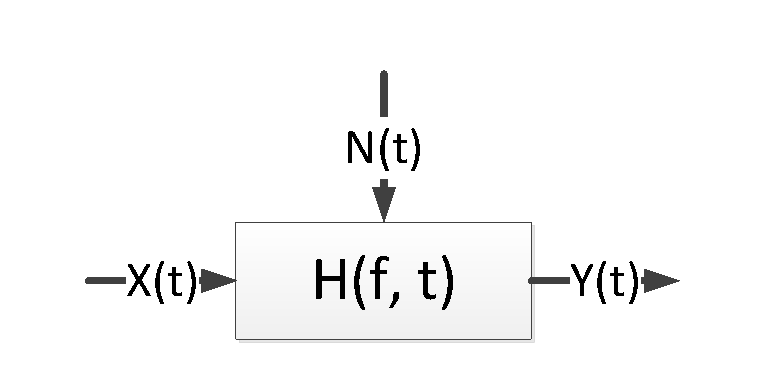
\includegraphics[width=0.5\textwidth]{pic/channel.pdf}
\end{center}
\begin{itemize}
	\item Представление $X(t), Y(t)$ сигналов в частотной области
	\item Полоса пропускания канала
	\item Свойства сигналов с ограниченным спектром
	\item Пропускная способность канала с ограниченной полосой пропускания (теорема Найквиста)
	\item Пропускная способность канала с шумом (теорема Шеннона)
\end{itemize}
\end{frame}
%--------------------------------------------------------------------------------
\subsection{Ряды Фурье и Преобразование Фурье}
%--------------------------------------------------------------------------------
\begin{frame}
\frametitle{Ряд Фурье и преобразование Фурье}
Периодическая функция может быть представлена в виде ряда Фурье:
$$
\nu (t) = \sum_{n=-\infty}^{\infty}C_n e^{j\cdot 2 \pi n f_0 t}, C_n = \int_{T_0} \nu (t) e^{-j\cdot 2\pi nf_0t}dt
$$
Для непериодических функций -- преобразование Фурье:
$$
F(f) = \frac{1}{\sqrt{2 \pi}}\int_{-\infty}^{\infty}\nu(t)\cdot e^{-j\cdot 2\pi \omega t}d\omega
$$
$$
f(F) = \frac{1}{\sqrt{2 \pi}}F(\omega)e^{j\cdot x\omega}d\omega
$$
\end{frame}
%--------------------------------------------------------------------------------
\begin{frame}
\frametitle{Свойства преобразования Фурье}
Умножению во временной области сопоставляется свёртка в частотной, и наоборот:
$$
f \cdot g \Rightarrow F \otimes G, f \otimes g \Rightarrow F \cdot G
$$
Свойство квантования времени:
$$
g\Big(\frac{t}{\tau}\Big) \Rightarrow |\tau|G(f\cdot \tau)
$$
Задержка сигнала приводит к набегу фазы:
$$
g(t-\tau) \Rightarrow G(f)\cdot e^{-j\cdot 2\pi f \tau}
$$
Преобразование Фурье обладает свойством дуализма:
$$
G(t) \Rightarrow g(-f)
$$
\end{frame}
%--------------------------------------------------------------------------------
\begin{frame}
\frametitle{Свойства преобразования Фурье}
Периодическое повторение сигнала во временной области приводит к выборке в частотной области:
$$
\sum_{n\in Z} g(t) \otimes \delta (t - n\tau) \Rightarrow \frac{1}{|\tau|}\sum_{n \in Z}\Bigg(G(f)\cdot \delta(f - \frac{n}{\tau})\Bigg)
$$
Периодическое повторение сигнала в частотной области приводит к выборке во временной области:
$$
\sum_{n\in Z} g(t) \cdot \delta (t - n\tau) \Rightarrow \frac{1}{|\tau|}\sum_{n \in Z}\Bigg(G(f)\otimes \delta(f - \frac{n}{\tau})\Bigg)
$$
Связано с тем, что преобразование Фурье от ``гребёнки'' из дельта-функций будет ``гребёнкой'' из дельта-функций
\end{frame}
%--------------------------------------------------------------------------------
\begin{frame}
\frametitle{Преобразование Фурье в передаче данных}
\begin{center}
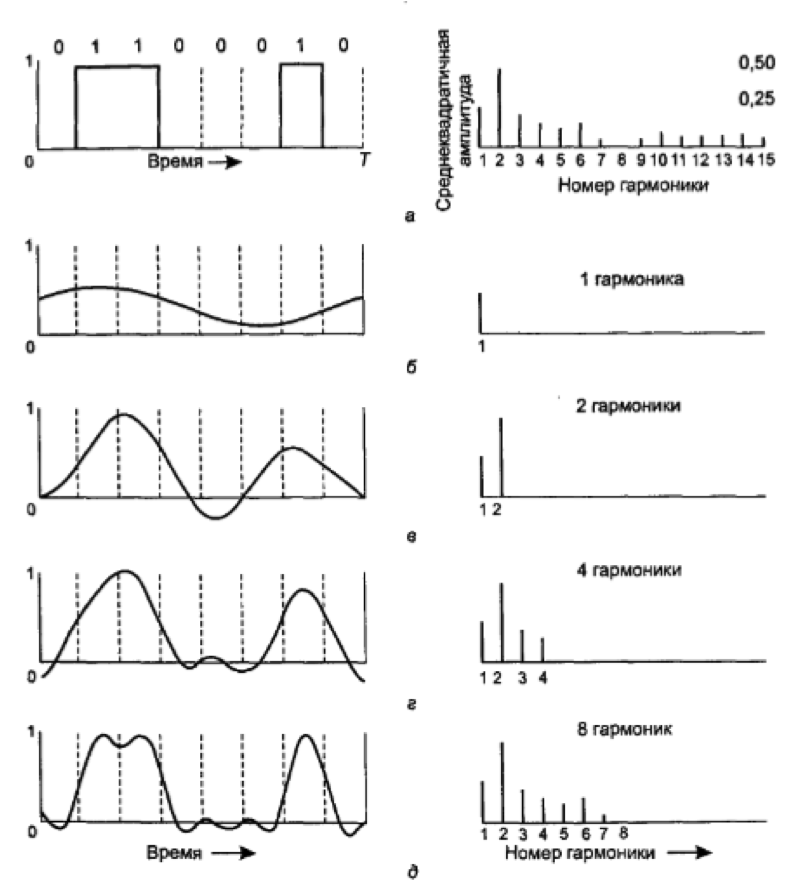
\includegraphics[width=0.6\textwidth]{pic/fourier.png}
\end{center}
\end{frame}
%--------------------------------------------------------------------------------
\begin{frame}
\frametitle{Преобразование Фурье в передаче данных}
Каналы передачи данных описываются АЧХ
\begin{itemize}
	\item Полоса пропускания – полоса частот, в которой затухание равно или менее заданного значения
	\item Частота среза – частота пропускания на которой затухание достигает заданного значения
	\item Как правило – учитывают затухание в 3 дБ, т.е. в два раза
\end{itemize}
Для беспроводных каналов АЧХ может иметь сложную форму, изменяющуюся во времени. Сложности передачи данных в беспроводном канале:
\begin{itemize}
	\item Частотная селективность беспроводного канала
	\item Существенные кратковременные ``замирания''
\end{itemize}
\end{frame}
%--------------------------------------------------------------------------------
\subsection{Электромагнитный спектр}
%--------------------------------------------------------------------------------
\begin{frame}
\begin{center}
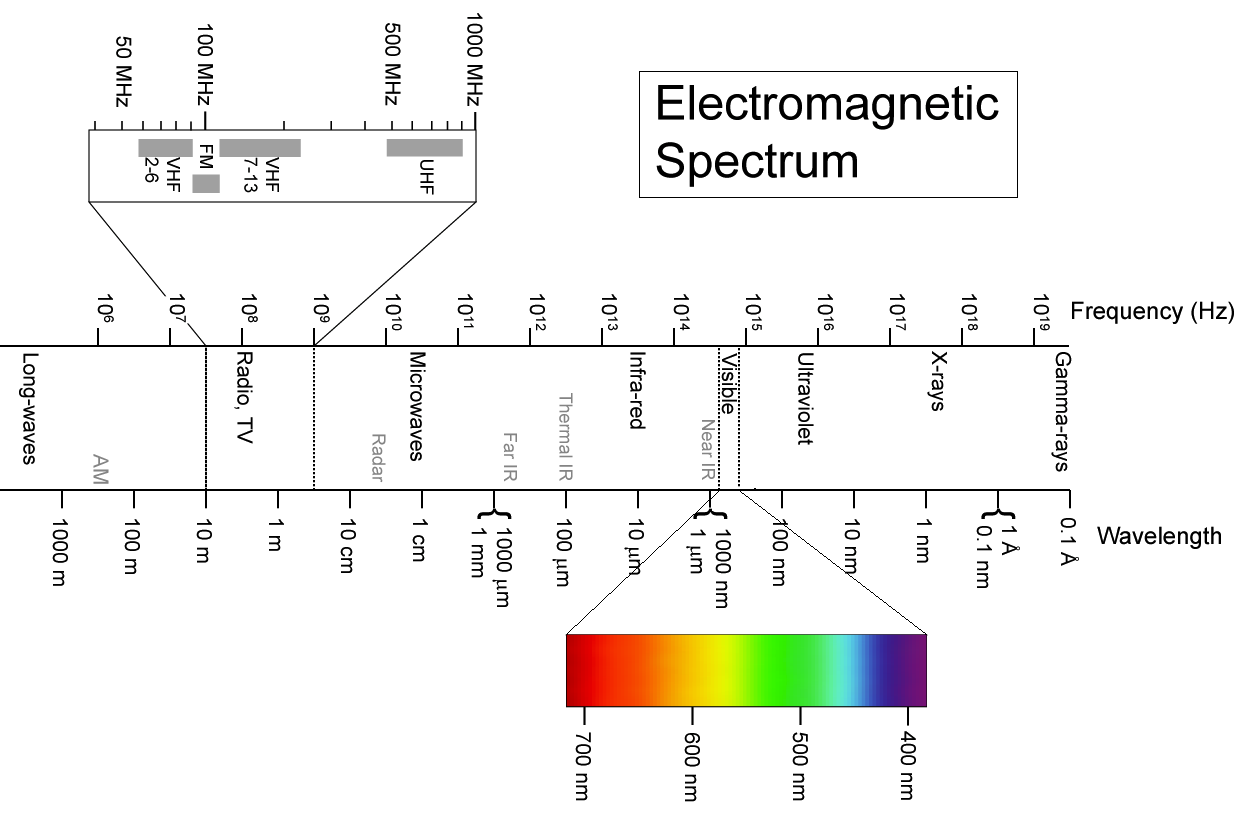
\includegraphics[width=1.05\textwidth]{pic/spectrum.png}
\end{center}
\end{frame}
%--------------------------------------------------------------------------------
\begin{frame}
\frametitle{Электромагнитный спектр}
\begin{itemize}
	\item Электромагнитный спектр -- дорогостоящий ресурс.
	\item Передача данных вне разрешённых частот -- нарушение закона.
\end{itemize}
Практически все системы передачи данных ограничены в спектре, им предоставляются каналы с \emph{ограниченной полосой частот}.

Дальнейшее изложение посвящено максимальной скорости передачи в канале с ограниченным спектром.
\end{frame}
%--------------------------------------------------------------------------------
\subsection{Сигналы с ограниченным спектром}
%--------------------------------------------------------------------------------
\begin{frame}
\frametitle{Дискретизация сигнала с ограниченным спектром}
В цифровых системах обработки сигналов сигнал представляется в виде отсчётов -- значений амплитуд сигнала в заданные моменты времени (с одинаковым шагом).

Свойство преобразования Фурье: Периодическое повторение сигнала во временной области приводит к выборке в частотной области:
$$
\sum_{n\in Z} g(t) \otimes \delta (t - n\tau) \Rightarrow \frac{1}{|\tau|}\sum_{n \in Z}\Bigg(G(f)\cdot \delta(f - \frac{n}{\tau})\Bigg)
$$
\end{frame}
%--------------------------------------------------------------------------------
\begin{frame}
Копии спектра не должны пересекаться
\begin{center}
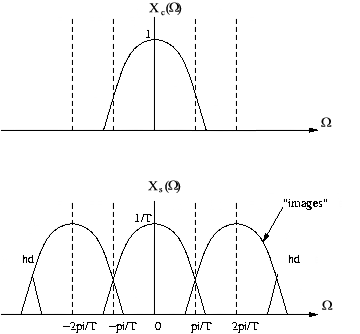
\includegraphics[width=0.4\textwidth]{pic/aliasing.png}
\end{center}
Шаг между копиями спектра - частота дискретизации.

Частота дискретизации -- удвоенная максимальная частота сигнала:
$$
f_{original} - f_{image} > \frac{2}{\tau} \Rightarrow f_{discretization} > \frac{2}{\tau}  = 2\cdot f_{max}
$$
\end{frame}
%--------------------------------------------------------------------------------
\subsection{Формула Найквиста}
%--------------------------------------------------------------------------------
\begin{frame}
\frametitle{Формула Найквиста (1)}
Предположим, что мы хотим каждые $\Delta T$ передавать одно вещественное число по каналу с ограниченной полосой. Каково минимальное $\Delta T$, при котором это возможно?
\pause
$$
\Delta T \geq \frac{1}{2\cdot B} \Rightarrow 2B \textrm{ вещественных чисел в секунду}
$$
\end{frame}
%--------------------------------------------------------------------------------
\begin{frame}
%\frametitle{Цифровая модуляция}
\begin{block}{Baseband signal}
Описание сигнала, частота которого изменяется от 0 до частоты среза -- информационный комплексный сигнал $z(t) = I(t) + j\cdot Q(t)$.
\end{block}
\begin{block}{RF-band signal}
Описание сигнала, частота которого изменяется в районе значения \emph{несущей} частоты.
$$
A_c(t) \cdot \cos (2\pi f_ct + \phi(t)) \textrm{ или } Re\{z(t)\cdot e^{jf_ct}\}
$$
\begin{itemize}
 \item [$A_c$] амплитуда
 \item [$f_c$] частота
 \item [$\phi$] фаза
\end{itemize}
\end{block}
\end{frame}
%--------------------------------------------------------------------------------
\begin{frame}
\frametitle{Модуляция}
\begin{enumerate}
 \item Способ представления потока бит в виде аналоговых сигналов
 \item Перенос сигнала на хорошо распространяющиеся частоты
\end{enumerate}
$$
I(t) = A_c(t)\cdot \cos(\phi(t)), Q(t) = A_c(t)\cdot \sin(\phi(t)).
$$
$$
A_c(t) \cdot \cos (2\pi f_ct + \phi(t)) = I(t)\cdot \cos (2\pi f_ct) - Q(t)\cdot \sin (2\pi f_ct),
$$
поскольку
$$
A_c \cdot \cos (2\pi f_ct + \phi) = A_c\cdot \cos (2\pi f_ct) \cos (\phi) - A_c\sin(2\pi f_ct)\sin(\phi)
$$
\begin{center}
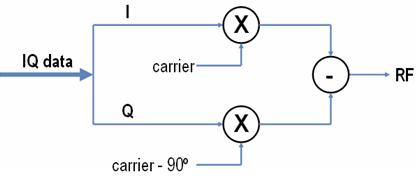
\includegraphics[width=0.5\textwidth]{pic/dhall_2_modulator.png}
\end{center}
\end{frame}
%--------------------------------------------------------------------------------
\begin{frame}
\frametitle{Формула Найквиста (2)}
Предположим, что данные передаются \emph{символами} длительностью T. По каналу передается комплексная $f(t)$ -- периодическая на  интервале $[0; T]$:
$$f(t) = \sum_{i=1}^{N}\alpha_i f_i(t)$$
\begin{itemize}
	\item Функции $f_i$ -- ортогональны на на интервале $[0; T]$ и периодические $\Rightarrow$ любая их линейная комбинация имеет ограниченный спектр.
	\item $\alpha_i$ -- комплексные числа. Передаваемый символ -- $\{\alpha_1,\ldots,\alpha_N\}$.
\end{itemize}
\end{frame}
%--------------------------------------------------------------------------------
\begin{frame}
\frametitle{Формула Найквиста}
Пусть дискретизация сигнала осуществляется с шагом $\tau$. Имея значения $f(t)$ в $\frac{T}{\tau}$ точках, мы можем определить коэффициенты $\alpha_i$.
Это возможно только тогда, когда система получаемых уравнений имеет решение, то есть мы имеем не более $\frac{T}{\tau}$ функций.
Какое максимальное количество функций $f_i$, то есть какое максимальное количество символов $a_i$ можно передать за время $T$?
$$
T/\tau = N \geq 2B \Rightarrow 2B \textrm{ комплексных чисел в секунду}
$$
\end{frame}
%--------------------------------------------------------------------------------
\begin{frame}
\frametitle{Формула Найквиста}
\begin{block}{Скорость Найквиста}
 Максимальное количество независимых символов в единицу времени
\end{block}
\begin{block}{БОД}
Количество независимых символов в единицу времени
\end{block}
\end{frame}
%--------------------------------------------------------------------------------
\begin{frame}
\frametitle{OFDM - частота символов равна частоте Найквиста}
Выполняется ли условие линейной независимости функций в приведённом примере?

Рассмотрим интервал $[-T, T]$, обозначим $f_0 = \frac{1}{2T}$ и рассмотрим набор комплексных функций:
$$
f_n(t) = e^{jf_0 nt}, F_n(f) = \delta (f - f_n), n=(-N\ldots N)
$$
\begin{itemize}
	\item Все функции ортогональны на этом интервале,
	\item для однозначного восстановления коэффициентов линейной комбинации необходимо $2N+1$ уравнений.
	\item ширина спектра, занимаемая сигналом равна $f_0 N$,
	\item скорость передачи (символов в секунду) равняется скорости Найквиста
\end{itemize}
\end{frame}
%--------------------------------------------------------------------------------
\begin{frame}
\frametitle{OFDM - ограниченность спектра}
\begin{center}
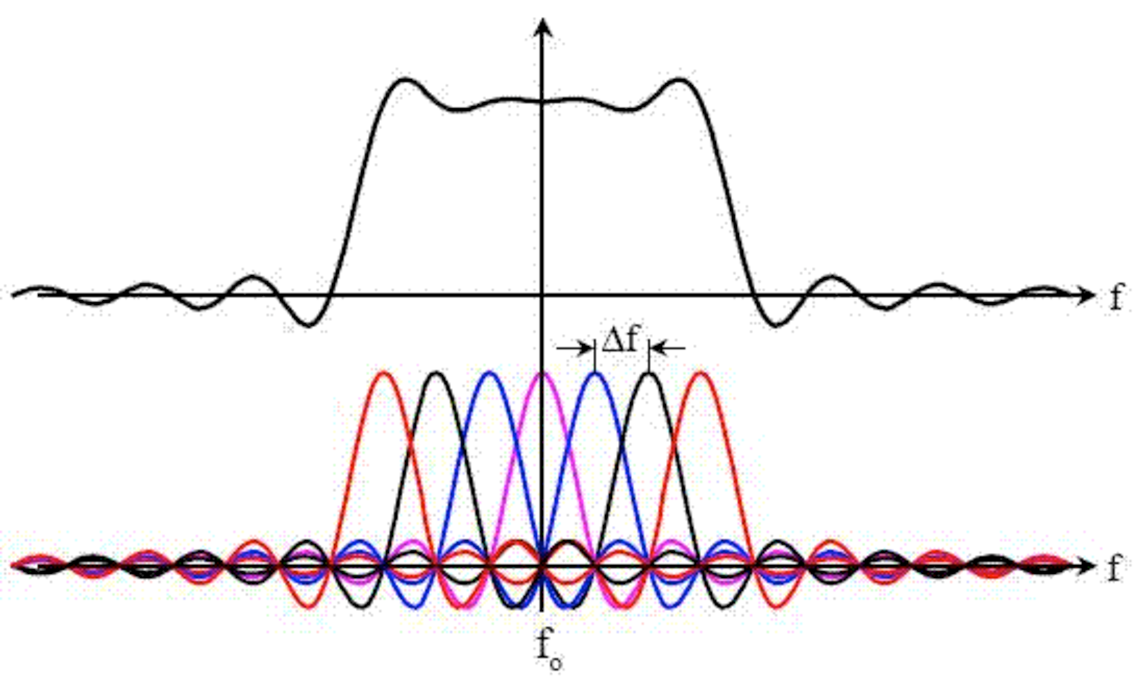
\includegraphics[width=\textwidth]{pic/ofdm-spectrum.pdf}
\end{center}
\end{frame}
%--------------------------------------------------------------------------------
\begin{frame}
\frametitle{Закон Хартли}
Пусть вместо вещественных чисел мы выбрали M значений сигнала, тогда пропускная способность канала без шума равна
$$
R\leq 2B\cdot \log_2 M \textrm{ (Формула Хартли)}
$$
Чем больше уровней сигнала мы выбрали -- тем больше канальная скорость.
\begin{itemize}
	\item Скорость передачи данных -- биты в секунду
	\item Скорость передачи символов - боды
\end{itemize}
Максимальное число уровней сигнала определяется соотношением сигнал-шум. Шум в канале ограничивает скорость передачи.
\end{frame}
%--------------------------------------------------------------------------------
\subsection{Теорема Шеннона}
%--------------------------------------------------------------------------------
\begin{frame}
\frametitle{Теорема Шеннона}
При соотношении сигнал-шум $\frac{S}{N}$ $M_{max} = \sqrt{1 + \frac{S}{N}}$
$$
R_{max} = B \log_2 (1+\frac{S}{N})
$$
Амплитуда и мощность связаны следующим соотношением:
$$
M = \sqrt{1 + \frac{S}{N}}
$$
\end{frame}
%--------------------------------------------------------------------------------
\section{Заключение}
%--------------------------------------------------------------------------------
\begin{frame}
\begin{block}{Стандартизация}
\begin{itemize}
 \item Международные организации по стандартизации
 \item Стандартизация Интернета
\end{itemize}
\end{block}
\begin{block}{Теоретические основы передачи данных}
 \begin{itemize}
  \item Ряды Фурье
  \item Спектр дискретизованного сигнала
  \item Скорость Найквиста
  \item Теорема Шеннона
 \end{itemize}
\end{block}
\begin{block}{Что читать}
 Таненбаум, главы 1 и 2.1.
\end{block}


\end{frame}
%--------------------------------------------------------------------------------
\end {document}
